% ****** Start of file apssamp.tex ******
%
%   This file is part of the APS files in the REVTeX 4.1 distribution.
%   Version 4.1r of REVTeX, August 2010
%
%   Copyright (c) 2009, 2010 The American Physical Society.
%
%   See the REVTeX 4 README file for restrictions and more information.
%
% TeX'ing this file requires that you have AMS-LaTeX 2.0 installed
% as well as the rest of the prerequisites for REVTeX 4.1
%
% See the REVTeX 4 README file
% It also requires running BibTeX. The commands are as follows:
%
%  1)  latex apssamp.tex
%  2)  bibtex apssamp
%  3)  latex apssamp.tex
%  4)  latex apssamp.tex
%
%
\documentclass[%
%  reprint,
 superscriptaddress,
%groupedaddress,
%unsortedaddress,
%runinaddress,
%frontmatterverbose, 
% preprint,
showpacs,preprintnumbers,
%nofootinbib,
%nobibnotes,
%bibnotes,
 amsmath,
 amssymb,
 aps,
 pra,
% prb,
% rmp,
%prstab,
%prstper,
%floatfix,
showkeys,
onecolumn,
% twocolumn,
notitlepage,
11pt,
% linenumbers,
tightenlines      % uncomment for double space
]{revtex4-1}

\usepackage[toc,page]{appendix}
\usepackage{float}
\usepackage{graphicx}% Include figure files
\usepackage{dcolumn}% Align table columns on decimal point
\usepackage{bm}% bold math
\usepackage{hyperref}% add hypertext capabilities
%\usepackage[mathlines]{lineno}% Enable numbering of text and display math
%\linenumbers\relax % Commence numbering lines

\usepackage[
% showframe,%Uncomment any one of the following lines to test 
% scale=0.7, 
% marginratio={1:1, 2:3}, ignoreall,% default settings
% text={4.8in, 8in},centering,
% text={6in, 8in},
centering,
a4paper,
margin=2.0cm,
% top=1.in,
% bottom=1.in,
% total={5.6in,8.75in}, % top=1.2in, left=0.9in, includefoot,
% height=10in,
a4paper,
% hmargin={3cm,0.8in},
% marginpar=1in,
% inner=1in,
% outer=1in,
% papersize={6.10in,9.25in}
]{geometry}

\usepackage{fontspec}

% \usepackage{cmbright}
% \DeclareFontShape{OT1}{cmss}{m}{it}{<->ssub*cmss/m/sl}{}
% \renewcommand{\rmdefault}{cmss}
% \renewcommand{\sfdefault}{cmss}

\setsansfont[
BoldFont=ArialBold.ttf,
BoldItalicFont=ArialBoldItalic.ttf,
ItalicFont=ArialItalic.ttf
]{Arial.ttf}
\renewcommand*\familydefault{\sfdefault} 
\setmainfont{Arial}


%%%%%%%%%%%%%%%%%%%%%%%%%%%%%%%%%%%%%%%%%%%%
%%%%%%%%%%%%%%%%%%%%%% COLOR %%%%%%%%%%%%%%%
%%%%%%%%%%%%%%%%%%%%%%%%%%%%%%%%%%%%%%%%%%%%
\usepackage{xcolor}
\usepackage{soul}
\definecolor{reddish}{HTML}{FBB4AE}
\definecolor{blueish}{HTML}{B3CDE3}
\definecolor{magentish}{HTML}{FF00AA}
\definecolor{greenish}{HTML}{a1d99b}
\DeclareRobustCommand{\red}[1]{{\sethlcolor{reddish}\hl{#1}}}
\DeclareRobustCommand{\flow}[1]{\noindent{\sethlcolor{greenish}\hl{\textbf{FLOW}  #1}}}

\usepackage{colortbl}% http://ctan.org/pkg/colortbl
\definecolor{GrayAbstract}{gray}{0.97}
\definecolor{Gray2}{gray}{0.85}
\definecolor{Gray}{gray}{0.95}

\DeclareRobustCommand{\blue}[1]{{\sethlcolor{blueish}\hl{#1}}}
\DeclareRobustCommand{\magenta}[1]{{\sethlcolor{magentish}\hl{#1}}}

% \linespread{1.} 
% \linespread{1.6}
        
%%%% modifying APS template a bit:
% times 
% \usepackage{mathptmx}
% arabic number section
\renewcommand\thesection{\arabic{section}}
\renewcommand\thesubsection{\thesection.\arabic{subsection}}
% section left-side and title style
\usepackage{titlesec}
\titleformat*{\section}{\Large\bfseries}
\titleformat*{\subsection}{\bfseries}
% FIG. -> Fig.
\renewcommand{\figurename}{Fig.}
% spacing after and before section headers
\titlespacing*{\section}{0pt}{1ex plus 1ex minus .5ex}{0.5ex}
\titlespacing*{\subsection}{0pt}{1ex plus 1ex minus .5ex}{0.5ex}
\usepackage{natbib}
\setcitestyle{sort&compress, super}
\definecolor{blueish2}{HTML}{0830Bb}
\hypersetup{colorlinks = true,
            linkcolor = blueish2,
            urlcolor  = blueish2,
            citecolor = blueish2,
            anchorcolor = blueish2}
% section left-side and title style


\makeatletter
\renewcommand*{\fnum@figure}{{\normalfont\bfseries \figurename~\thefigure}}
\makeatother

\setlength{\bibsep}{2mm}
\setlength\bibhang{0.1in}
\usepackage{setspace}
\begin{document}

\title{\Large Machine Learning to Study Patterns in Chess Games}

% \author{NO AUTHORS GIVEN}
\author{Isaac Cheng}
\email{isaaccheng9@gmail.com}

\begin{abstract}
\noindent \textbf{Abstract}

% \textnormal{
\noindent 
(100-200 words)

\end{abstract}

\maketitle

\vspace*{\fill}


\begin{center}
I certify that all material in this dissertation which is not my own work has been identified.
\end{center}
\vspace{1em}

Signature: \hrulefill


\newpage
\section{Introduction}
The use of computers in chess has been a popular topic of study over the past century. Computers are able to perform tasks sequentially incredibly quickly, they generally do not make mistakes, and they have a large capacity for storing information quickly in the form of secondary storage devices. In chess, this means they are able to perform move calculations at orders of magnitudes faster than humans, and they can store large amounts of information about chess games.

Strategic board games are good candidates for artificial intelligence research due to their fixed environment. Other games like Go have also undergone extensive studies \cite{muller2002computer}. Chess is an apt game for data mining and machine learning -- the games are well-structured, with a defined search space and comprehensive databases of historical chess games. Literature on chess strategy is centuries-old, but the terabyte-scale exploration of games has only caught on recently. Professional players have started to improve their game using analytics tools like Stockfish, and platforms like Lichess and Chess.com have integrated such tools to make them more accessible to everyone.

Over the past decade, chess has become increasingly significant in popular culture. The rise of full-time streamers on platforms like Twitch has made chess a mainstream form of entertainment. Sponsors have invested substantial sums of money into chess, with platforms such as Chess.com incentivising streamers to integrate the game into their schedules. The onset of the COVID-19 pandemic further encouraged this, with people exploring digital forms of entertainment due to lockdown mandates from governments across the globe. 'The Queen's Gambit' was released in 2020, serving as the most poignant example of chess in popular culture yet. People started to take a greater interest in the game, and the number of games played daily on online platforms like Chess.com and Lichess has skyrocketed. 

The study of chess has great social importance, as chess games involve cognition and human behaviour that we can apply more generally. For example, social learning theory is a crucial aspect of chess strategy -- players building their chess fundamentals learn from the same material and are thus likely to develop homogeneous habits. People have researched the impact of social learning in the game of Go \cite{beheim2014strategic}, but not for chess. In this project, I will apply data mining and machine learning tools to millions of chess games to understand patterns in how people play chess.

\section{Preliminary Research}

\subsection{Early History of Computer Chess}
Since the first digital computer was switched on 1945, programmers have sought to build a machine that could defeat the world chess champion \cite{earlyComputerChessHistory}. In 1948, Alan Turing worked with David Champernowne (an economist and mathematician) to create a machine routine for playing chess, dubbed the 'Turochamp' \cite{copeland2005turing}. They did not have a machine, so they simulated the machine's behaviour by hand with a pen and pencil \cite{copeland2005turing}. Champernowne reported that his wife, who was a beginner at chess, took on the machine and lost \cite{copeland2005turing}. A year later in 1949, Claude Shannon wrote a paper that described a computer that could play chess -- his idea was to focus on analysing the seven most likely moves from the current position, and branching from each of these positions into the next seven most likely replies from the opposition, and so forth until the computer runs out of memory \cite{shannon1950xxii}. The first chess program was eventually implemented in November 1951 by Dietrich Prinz. However, unlike Turing's Turochamp, Prinz's program could not complete a full game of chess and used exhaustive search to play moves rather than a heuristic \cite{copeland2005turing}.

The first computer to beat a world champion was IBM's Deep Blue, which defeated Garry Kasparov over a six-game match in 1997 \cite{seirawan1997implications}. Deep Blue was a supercomputer that was able to perform 200 million calculations per second \cite{strogatz2018one}. It was the first computer to use a heuristic search algorithm, which is a method of searching for a solution to a problem by evaluating possible solutions and choosing the best one. By this point, chess engines were stronger than human players, yet they still lacked a deep understanding of the game. Deep Blue's victory was accredited to its brute-force ability -- its over-reliance on this was demonstrated in the first game of their match, as it sacrificed Kasparov's sacrifice of a rook for a bishop, only to lose 16 moves later \cite{strogatz2018one}.

\subsection{Modern Developments in Computer Chess}
Stockfish is currently the strongest chess engine in the world \cite{computerChessRatingLists}. It is used by many professional players to analyse their games, with Chess.com and Lichess also using Stockfish to provide game analysis on their platforms. It is a free, open-source chess engine that started with the open-source Glaurung engine, which was authored by Tord Romstad. The first version, Stockfish 1.0, was released in November 2008 when Marco Costalba took over the Glaurung 2.1 code \cite{aboutStockfish}. It started to gain prominence from their Stockfish 3 release in 2013, in which they started using a distributed testing framework called Fishtest \cite{fishtestDistributedTestingFramework}. This was a web application written in Python that allowed volunteers to donate CPU time to test improvements to the engine. They used Fishtest to test whether changes to the game-playing code demonstrate statistically significant improvements to the engine, using the chi-squared test to verify tests on the framework. Twelve months after the inception of Fishtest, Stockfish skyrocketed to the top of chess engine rating lists, gaining 120 Elo points \cite{stockfishRatingsAfterFishtest}. As of November 2022, users have contributed over 9580 years of CPU time to the project, playing over 5.5 billion chess games \cite{fishtestUsers}. 

Stockfish uses the alpha-beta pruning search algorithm, which improves minimax search \cite{v1928theorie} by avoiding variations that will never be reached in optimal play because either player will redirect the game \cite{maharaj2022chess}. Due to the number of possible moves at each position, it is computationally infeasible to search every tree subgraph until the end of the game, so Stockfish finishes its search once it reaches a certain depth. This is measured in ply, which measures the distance between the root node and the leaf nodes \cite{maharaj2022chess}. Stockfish uses iterative deepening to incrementally increase the depth of its search tree \cite{de2014thought}. Despite this, it does not necessarily search all the moves in this search space -- Stockfish uses heuristics to search promising variations in more depth than normal, and less promising variations in less depth than normal \cite{maharaj2022chess}. The engine uses forward pruning to reduce the search space via futility pruning -- if the evaluation of a position is significantly worse than the player's alternative, it prunes the position's children early \cite{maharaj2022chess}. It also uses reduction techniques, which involves searching tree subgraphs to lower depths rather than completely omitting them from the search \cite{maharaj2022chess}, such as late move reductions -- this assumes that the engine checks better moves earlier, so it searches later moves with less depth in the move tree \cite{levy1989sex}. Once Stockfish's search algorithm arrives at a leaf node, it applies a heuristic evaluation function to determine whether it favours white or black \cite{maharaj2022chess}. Since Stockfish 11, it uses NNUE (Efficiently Updatable Neural Networks) evaluation \cite{nasu2018efficiently}, a neural network that is trained to predict the output of the classic Stockfish evaluation function using basic inputs using the previous evaluations of millions of positions at moderate search depth \cite{stockfishNNUEEvaluation}. NNUE's architecture is optimised for speed on CPU machines, and it uses a shallow, fully connected network with four hidden layers \cite{guideToStockfishNNUE}. The input layer of binary features describes the position of the white and black king relative to the white and black pieces, and dimensionality reduction is performed by passing the board feature vector through two hidden layers and an output layer -- this results in a final scalar value for position evaluation \cite{maharaj2022chess}.

Researchers at DeepMind have developed their machine-learning algorithms to master chess alongside other strategic games such as shogi and Go with their AlphaZero machine-learning algorithm \cite{silver2018general}. It was based on their recent AlphaGo Zero program, which achieved superhuman performance using an algorithm based solely on reinforcement learning, with no human data, guidance, or domain knowledge beyond the rules of Go \cite{silver2017mastering}. Likewise, AlphaZero started with no knowledge of chess (nor any of the other strategy games) beyond the basic rules and became the best chess player (human or computer) in the world within hours of learning by playing millions of games \cite{strogatz2018one}. AlphaZero's chess abilities were tested by playing against Stockfish. AlphaZero was able to beat Stockfish 8-0 in a match of 8 games \cite{silver2018general}.

AlphaZero's victory was attributed to its ability to learn from its mistakes, which is a key aspect of machine learning. It implements a general-purpose Monte Carlo tree search (MCTS) algorithm rather than minimax, which Stockfish uses \cite{silver2017mastering2}. MCTS is a heuristic search algorithm based on the idea is that when a player selects their actions randomly, very little can be inferred from a single game, but a good strategy can be found by simulating a multitude of random games \cite{chaslot2008monte}. It expands the search tree based on random sampling of the search space and performs playouts, where each game is played to the end via random move selection. The results of each game is used to weight the nodes in the game tree to make better nodes more likely to be chosen in the future -- after some number of simulations, the child node with the most samples is chosen \cite{chaslot2008monte}. Whereas minimax and alpha-beta pruning algorithms are serial in nature, MCTS is parallel, as the random sampling of the search space can be performed in parallel \cite{silver2017mastering2}. Hence, MCTS can use batching on GPUs to speed up the search process, which is fundamental to AlphaZero's success.

Stockfish and AlphaZero represent the current state of the art in computer chess. While DeepMind have not open sourced AlphaZero, a project 'LCZero' was born as an attempt to reproduce it using crowd computing \cite{maharaj2022chess}. This predominantly uses the same search and evaluation techniques as AlphaZero, but with some improvements that improve the strength of the engine. Stockfish's strength lies in its search, whereas LCZero's strength is in its evaluation. This has led to performance comparisons between Stockfish and LCZero using Plaskett's Puzzle, a chess endgame study known to be an anti-engine puzzle. Stockfish searched through nearly 1.9 billion positions using its minimax algorithm, and its domain-specific search optimisations helped it to reach the optimal solution. However, LCZero's search algorithm was unable to find the optimal solution as it chose the wrong lines to search deeply \cite{maharaj2022chess}. Part of this can be attributed to the fundamental differences between the engines -- LCZero was built from zero knowledge of the game except the basic rules of chess, whereas Stockfish uses chess-specific search heuristics. Thus, Stockfish is stronger than LCZero, but LCZero is more generalisable and can be applied to other strategy games like shogi and Go.

\subsection{Relevance of Computer Chess}
The patterns that computer chess engines like Stockfish and AlphaZero learn are similar to those that humans learn. This is because the search algorithms used by these engines are based on the same principles as search techniques used by humans. Stockfish's futility pruning method is similar to the way humans implicitly prune search trees -- if a move is unlikely to be optimal, then it is unlikely to be optimal in the future, and so the search can be pruned. Meanwhile, AlphaZero's MCTS algorithm is similar to how humans use their memory of historical games to make decisions in the future -- if they recognise a similar position to one they have seen before, they can use their memory of the outcome of that game to infleunce their decision. If they achieved a positive outcome from their previous move, they are more likely to make the same move again, whereas they are likely to change their strategy if they achieved a negative outcome.

These similarities between human and computer chess are important -- although we are not creating a chess bot, we will consider the patterns for the basis of our investigations. Part of the analysis in our project could involve quantifying the extent of how historical results affect the likelihood of a chess opening being played, as opposed to players simply playing the most well-known openings. While the latter has little to no influence on computer chess, the former is likely to be an aspect of human chess to different degrees according to player demographic.

\subsection{Practical Use of Chess Databases}
Most recently, computer chess has come under scrutiny in chess tournaments, as US Grandmaster Hans Niemann was involved in a cheating scandal when he defeated reigning five-time World Chess Champion Magnus Carlsen in the third round of the 2022 Sinquefield Cup \cite{niemannDefeatsCarlsen}. Carlsen withdrew from the cup the next day on 5 September 2022, posting a tweet implying an accusation that Niemann was cheating over the board, an accusation that Niemann denied \cite{niemannCheatingAllegations}. In a follow-up tweet on 26 September 2022, Carlsen accused Niemann of cheating, stating his belief that Niemann cheated more often and more recently than he publicly admitted \cite{niemannCheatingAllegations2}. Chess.com conducted an investigation into Niemann's games and banned the player from their platform, publishing a report on 4 October 2022 alleging that Niemann likely received illegal assistance in more than 100 online games, as recent as 2020, including contests in which prize money was on the line \cite{niemannCheatingChessComReport}. They used a variety of analytics tools designed to detect cheating, including tools that compared the moves he made to the moves recommended by the top chess engines \cite{niemannCheatingChessComReport}. An independent investigation was conducted by Kenneth Regan, a professor of computer science at the University of Buffalo, whom is paid by The International Chess Federation (FIDE) to monitor tournaments \cite{niemannCheatingReganReport}. He also concluded that Niemann was likely cheating, based on the results of his proprietary cheat detection software that calculates the odds that a player of a given skill level can make a given set of moves \cite{niemannCheatingReganReport}. Similar to part of Chess.com's investigation, Regan's software compared Niemann's moves to the moves recommended by the top chess engines and used a statistical model to output a z-score representing the degree of similarity between the player and the engine \cite{niemannCheatingReganReport}. Hans Niemann filed a \$100 million defamation lawsuit against Magnus Carlsen and Chess.com amongst others for 'colluding to blacklist' Niemann from the chess world \cite{niemannCheatingDefamationLawsuit}. The case is ongoing at the time of writing in November 2022, but the scandal has highlighted the influence that computer chess has in the modern game, both in terms of its ability to cheat and its ability to analyse games for investigation purposes.

This saga demonstrates the practical use of chess databases, as we will use them to find patterns in how people play chess and these patterns can be used to identify players who are cheating. While we will not be creating the cheat detection algorithms themselves (as sophisticated programs like Lichess' Irwin AI Hunter already exist \cite{lichessIrwinCheatDetection}), the patterns that we find could be used to create or improve such algorithms. For example, we could cluster players by their playstyle using metrics such as tendency to sacrifice pieces, and then these clusters could be used to flag players who are playing abnormally. Similarly, we could analyse games to determine the parameter space of chess players on x and y-axes, and this could flag players who demonstrate abilities beyond the wider chess population for further investigation.

\subsection{Chess Piece Valuation}
In chess, the value of a piece is determined by its ability to influence the outcome of the game. The standard valuation system assigns 1 point to a pawn, 3 points to a knight, 3 points to a bishop, 5 points to a rook, and 9 points to a queen. However, these points are fixed and do not consider the position of the pieces on the board -- a well-positioned bishop defending multiple pieces may be more valuable than an inactive rook that is passively positioned in the corner despite technically having a lower valuation. Furthermore, certain pieces combinations are generally thought to be more valuable than the sum of their parts. For example, two bishops are considered more valuable than a bishop plus a knight \cite{timoshchenko1993bishop}. DeepMind have also used self-play games with AlphaZero to fit a linear model that predicts the outcome of games solely from the difference in piece material, and ended up with 1 for a pawn, 3.05 for a knight, 3.33 for a bishop, 5.63 for a rook, and 9.5 for a queen \cite{tomavsev2020assessing}. Edward Lasker presented the idea of pieces having different valuations at different points of the game -- in the middle game, he gave 1 point to a pawn, 3.5 to a knight, 3.5 to a bishop, 5.25 to a rook, and 10 to a queen \cite{lasker2021chess}. This is something that we could investigate in our project, as we could use the data from our chess databases to determine the value of pieces at different points of the game based on the win rate of the player who has the advantage of the piece.

\subsection{Growth in the Popularity of Chess}
While there has been continuous growth in the popularity of chess over the last decade, a significant spike occurred with the pandemic and the release of 'The Queen's Gambit'. Some people have researched Lichess databases to demonstrate this, such as in the chessOpeningStats repository (see figure 1). However, there is a lack of formal academic research on this topic -- the closest is a thesis that investigates the influence of Beth and their qualitative effects on how viewers in the Netherlands and United States view chess \cite{lowie2021big}, but this does not provide quantifiable results.

\begin{figure}[h]
    \caption{Popularity of Lichess in Number of Games Played Daily \cite{chessOpeningStats}}
    \begin{center}
    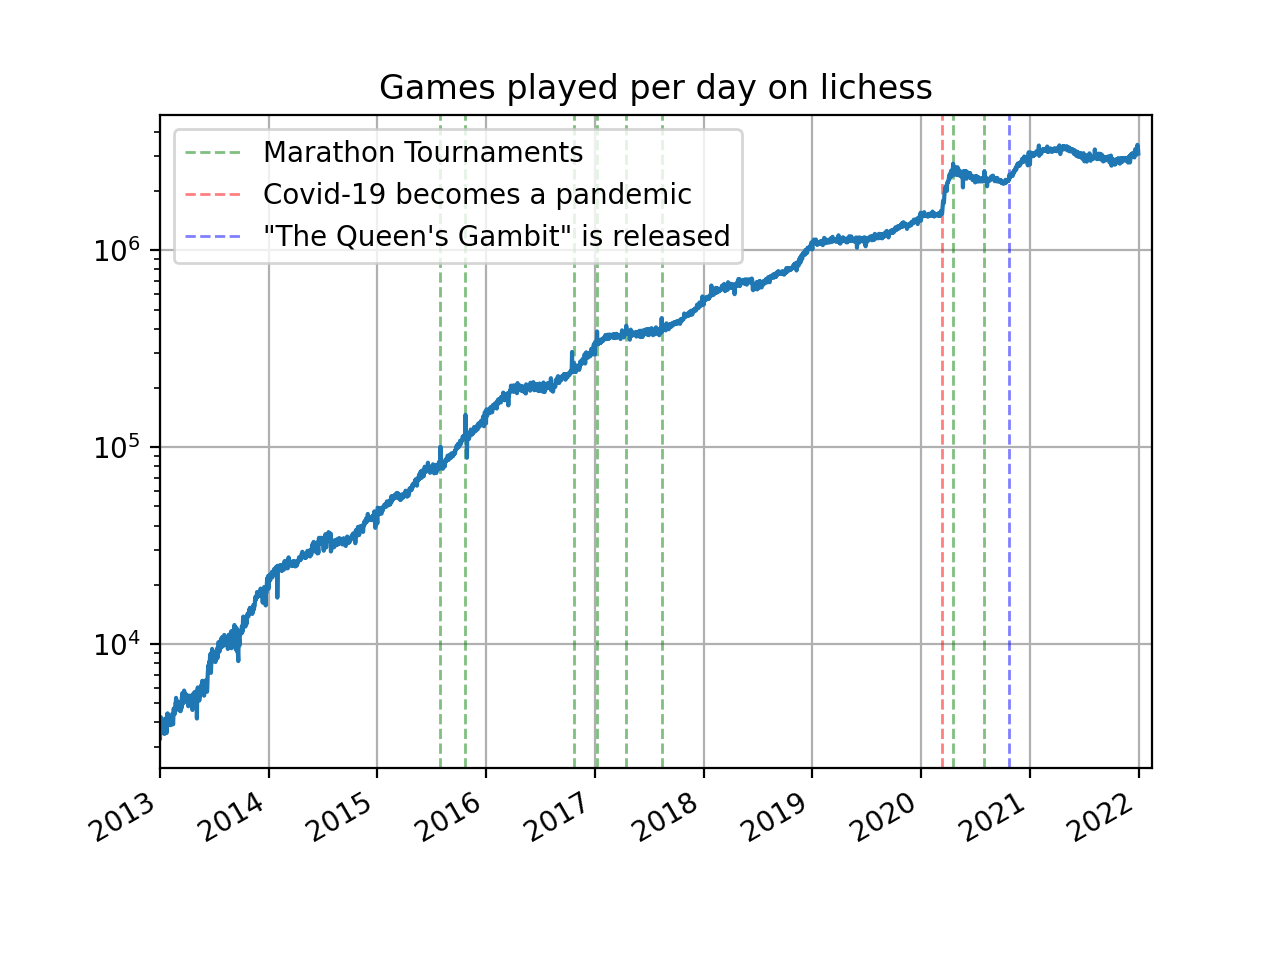
\includegraphics[width=0.6\textwidth]{images/Lichess Number of Games Played Per Day.png}
    \end{center}
\end{figure}

\section{Project Aims and Objectives}
Machine learning in chess covers a broad range of topics, so it is crucial to scope design and development systematically. We will start exploring simple, wide-spanning areas to build a baseline -- this may include answering questions such as:

\begin{itemize}
    \setlength\itemsep{0em}
    \item What are the most common chess openings and their success rates?
    \item How effectively does the centipawn score of a game predict the outcome of the game?
    \item What is the distribution of Elo ratings for online chess players?
\end{itemize}

Then, we will build up to more complex questions using previous findings. Questions may include:
\begin{itemize}
    \setlength\itemsep{0em}
    \item To what degree is social learning theory evident in chess?
    \item How good are existing metrics for predicting win probability in chess games?
    \item Can we determine more precise valuations for chess pieces at different Elo ranges based on win rates?
\end{itemize}

It is also important to outline what will be out of the project's scope. There is a vast range of chess game variants like Chess960 (also known as Fischer random chess), King of the Hill, and Antichess \cite{lichessBlitzRatingDistribution}. However, they would all introduce significant overhead to our research as they change the fundamental rules and theories of the game. In addition, the sample sizes for these games is much smaller -- there were only 337,940 games played on Lichess in October 2022 \cite{lichessOpenDatabase}. We will not include them in the project to avoid scope creep and to maintain a strong focus on the standard variant. In addition, we will not be creating a chess bot that plays games -- we will instead focus on generating insights to understand patterns in chess strategy.

\section{Project Management}

% \subsection{Overview of Plan}
% \begin{center}
%     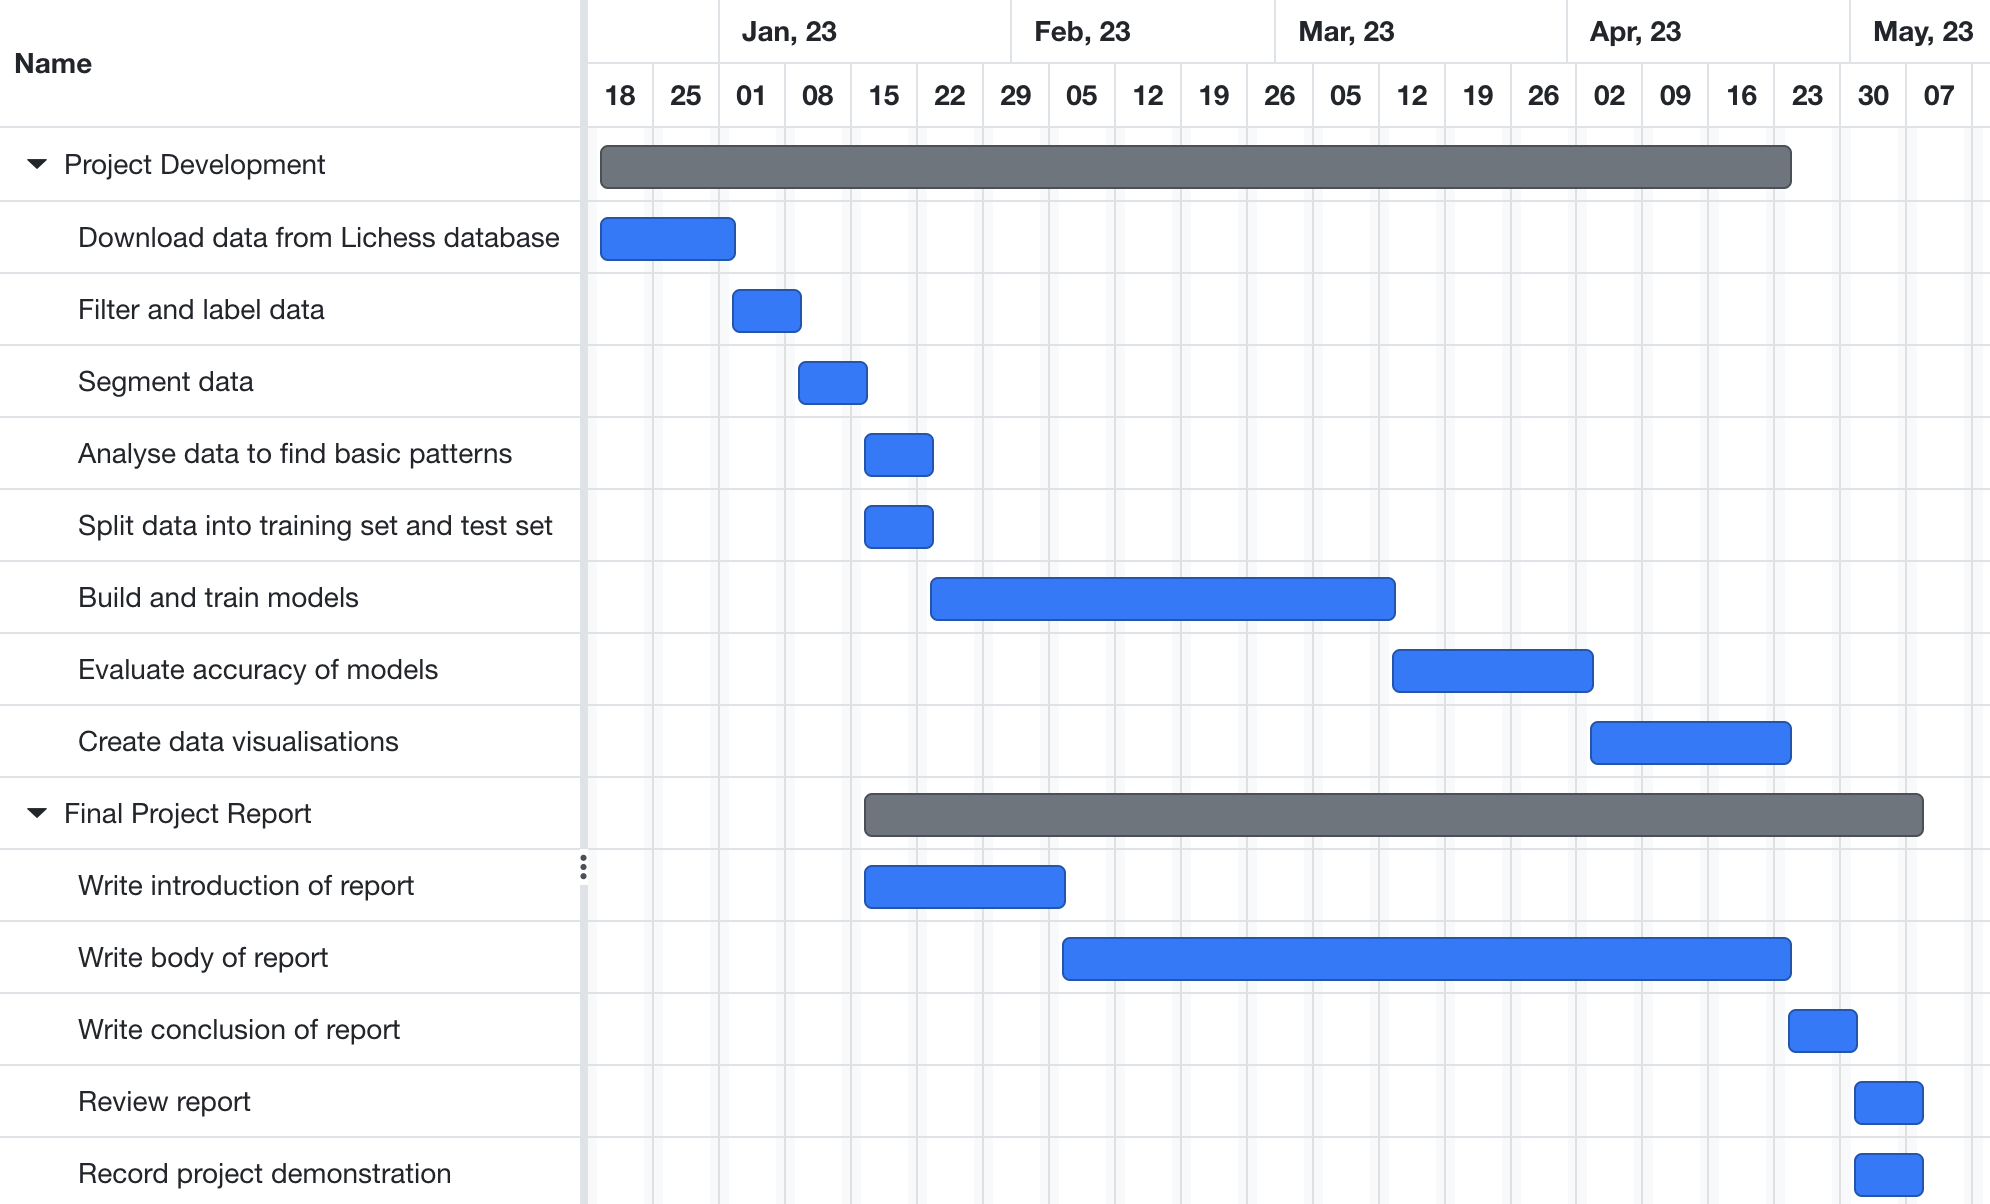
\includegraphics[width=0.8\textwidth]{images/Gantt Chart - Project Management.png}
% \end{center}

\subsection{Planning Our Approach}
A large data set is paramount to performing machine learning effectively. We will be using Lichess as our data source. They provide an open database of standard-rated games played on lichess.org every month in PGN (Portable Game Notation) format \cite{lichessOpenDatabase}, which is the standard for recording chess games \cite{pgnExplanation}. Lichess is one of the two mainstream platforms for playing chess online (alongside Chess.com), which means they provide a large sample to analyse each month -- October 2022 includes over 92 million standard rated games.

We will use Python 3.11.0 because Python is the de facto standard for data science \cite{pythonForDataScience} and that is the latest version at the time of writing. The python-chess library has emerged as the most popular for PGN parsing alongside other features -- it has over 1,900 stars on GitHub and is maintained regularly \cite{pythonChessLibrary}. It will accompany the Python Stockfish library, the best and most popular chess engine available to the public \cite{aboutStockfish} -- this enables us to integrate the Stockfish engine with Python to analyse positions and generate insights. In addition, we will use industry-standard Python libraries such as seaborn for graph visualisations, pandas for data frames, and NumPy for mathematical analysis.

To see an overview of my project plan, see appendix A.

\subsection{Project Risks}
There are very few risks in the project. The main risk is that the data set is not large enough to provide meaningful insights. However, this is unlikely to be an issue as Lichess provides a large data set every month, and there is already a history of monthly data from January 2013 onwards. The file sizes for Lichess' latest monthly data sets are huge, measuring at 30 GB for the compressed October 2022 download, and 214 GB when uncompressed. The computational analysis for this project will take place on my personal laptop, which is an M1 Max MacBook Pro 16 (2021) with 32 GB of RAM and 1 TB of SSD storage. If the lack of storage space becomes an issue when analysing multiple months' worth of data sets, we could look at using high-speed external solid state drives or using another machine. The latter solution would involve a high-performance desktop computer running a Linux distribution provided by my supervisor Chico Camargo, which could provide further benefits such as more powerful GPU accelerated computation to streamline our process.

Another risk is that the data set is not representative of the entire chess community. However, this is unlikely to be an issue as Lichess is one of the two mainstream platforms for playing chess online (alongside Chess.com), which means they provide a large sample to analyse each month. Lichess is a free platform, which means that it is accessible to a wide range of people. While it would be ideal to also obtain games from Chess.com to cover the two main platforms, this is infeasible as they do not provide an open database like Lichess.

\subsection{Legal and Ethical Issues}
There are a few legal and ethical considerations in the project, but none of them are of real concern. A potential legal issue could arise from Stockfish, which is licensed under the GNU General Public License (GPL) v3.0 \cite{stockfishRepository}. This means that we must make the source code for our project available to the public, which is not an issue as we will be using GitHub to host our project.

Furthermore, there may be concerns about the ethics of using machine learning to analyse chess games. However, this is not an issue as the data set is publicly available and does not contain any personal information. While the data set that we will analyse contains information about specific chess games and the usernames of the players, it does not contain any personally identifiable information (PII) such as names, addresses, or phone numbers. The output of our project will only concern chess strategy rather than the strategy or habits of individual players, and it will consist of highly aggregated data to find general trends. As our project will not create a chess bot that plays games, there is no risk of it being used to cheat in chess tournaments, which is a common concern with machine learning in chess.

\subsection{Downloading the Data}
Downloading the data is a straightforward process. As aforementioned, we will download monthly games from the Lichess Open Database (provided in compressed form), extract the games from the PGN file, and load them using python-chess. This library will enable us to read the game and navigate to the part we want to analyse. We will start by navigating to the final position of the games. Then, we will get the FEN (Forsyth-Edwards Notation) string, the standard notation for describing a chess game's board position \cite{pgnSpecification}. 

\subsection{Preparing the Data}
Once we have the position, we will analyse it using the Stockfish library. It provides information from the game, including the centipawn score. Stockfish computes the centipawn score using static evaluation of the board position and applying the mini-max algorithm and alpha-beta pruning \cite{maharaj2022chess}. It measures white's advantage, where a centipawn equals 1/100 of a pawn \cite{centipawnDefinition}. Hence, a score of 100 means that white has a pawn's worth of advantage, whereas a score of -100 indicates a pawn's advantage for black. If a player has a significant advantage, Stockfish may find a forced mate -- this means that one player can checkmate the other, regardless of the other player's moves. In this case, it will represent the score with either '\#{x}' or '\#{-x}', where x is the number of moves from a checkmate -- the former means white can checkmate black, and the latter means black can checkmate white. Note that this also includes 0 if the game ended due to a checkmate occurring on that move.

Before performing data analysis on the results, we will filter and label the data according to how the game ended. This is important because the most popular game modes in Lichess are timed (Bullet/Blitz/Rapid) as opposed to untimed (Classical) -- as of 24 November 2022, there were over 350,000 Bullet players, 700,000 Blitz players, and 400,000 Rapid players as compared with around 45,000 Classical players in the past week \cite{lichessBlitzRatingDistribution}. In timed games, a player loses the game when they run out of time regardless of their position. It is a particularly common situation in Bullet games that a player loses on time despite having an advantageous position on the board -- players are usually only given one or two minutes over the span of the game to make their moves, which poses a distinct challenge. This is an example of the types of games we may want to filter out, as they add unnecessary noise to the data.

Next, we will segment the data, as patterns could be found in different subsets of games based on the game mode. Games with shorter time limits in general may have different patterns to others, as time management skills become a more significant factor. For example, this factor would be more significant in a 5+0 Blitz game compared to a 10+0 Rapid game. We will also differentiate between games that ended from checkmate and games where a player resigned -- the former may be more indicative, as a player resigning is effectively extrapolating the rest of the game and deciding that they will lose when they may in fact be in a winning position.

To ensure that our machine learning models will be able to generalise, we will split the data into a training set and a test set. A common approach is to use the large majority as training data, typically 80\% of the data. The rest will be used as the testing data. We will use the training data to train our model, and the testing data to evaluate its performance. This will allow us to determine whether our model is overfitting or underfitting the data. If it is overfitting, we will need to reduce the complexity of the model, and if it is underfitting, we will need to increase it.

\subsection{Analysing the Data}
Once the data has been prepared, we will analyse the data to find patterns and investigate our questions. The basic patterns that we find will provide the foundation for our investigations and may not require machine learning, whereas investigating the complex questions that form the bulk of our project will involve it.

Finding the distribution of Elo ratings on Lichess will provide us a baseline for investigating social learning theory in chess. The distribution of Elo ratings is likely a normal distribution, and our initial hypothesis is that social learning theory will be more prevalent in lower and middle sections of the distribution -- people who are less skilled at chess may be more likely to copy the moves of others, whereas people who are more skilled may be more likely to play their own moves. Identifying the degree to which social learning theory is evident in chess may become a feature importance problem. A reasonable hypothesis is that social learning theory takes place to a greater degree for popular openings, as there is substantially more educational material for them. Thus, we could use feature selection methods such as information gain and variance thresholding to identify the features of games containing less popular openings.

Meanwhile, we could cluster games based on the type of moves that are played using k-means clustering. This will allow us to identify the most common types of moves, and we could use this to investigate whether there is a correlation between the type of move and the outcome of the game. For example, we could investigate whether a player is more likely to win if they play a positional move as opposed to a tactical move. This may also be a feature importance problem, as we could use the same feature selection methods as above to identify the features that are most indicative of the outcome of the game. On a similar note, we could cluster games as either open, which is when pieces can move freely and there are few pieces on the board, or closed, which is when pieces are restricted and there are many pieces on the board. Bishops are considered to be better in open games whereas knights are better in closed games, so we could seek to quantify the difference between these two pieces by calculating their respective piece values based on win rate in open and closed games.

We could also use logistic regression to determine whether there is a relationship between the centipawn score of a game and whether it ended in a checkmate or a resignation. This will allow us to determine whether there is a correlation between the two, and if so, whether it is a positive or negative correlation. It would form part of our investigation into how good the existing metrics for predicting win probability in chess games are.

\subsection{Evaluation}
We will also use cross-validation to ensure that our model generalises well to new data. This will involve splitting the data into k folds, where k is a number that we choose. We will then train the model k times, each time using a different fold as the testing data and the rest as the training data. In the end, we will average the results to get a more accurate estimate of the model's performance.

As this project focuses on using machine learning to analyse chess games, we will evaluate the performance of our models using metrics that are relevant to machine learning. This starts with the confusion matrix, which counts the number of true positives, true negatives, false positives, and false negatives. Based on the confusion matrix, we will measure accuracy, precision, recall, F1 score, and receiving operating character (ROC) curve to evaluate the performance of our models.

\begin{itemize}
    \item Accuracy is the proportion of correct predictions, defined as: $\frac{\text{number of correct predictions}}{\text{number of data points}}$
    \item Precision is the proportion of positive predictions that are correct, defined as:
    
    $\frac{\text{number of true positives}}{\text{number of true positives + number of false positives}}$
    \item Recall is the proportion of positive cases that are correctly identified, defined as:
    
    $\frac{\text{number of true positives}}{\text{number of true positives + number of false negatives}}$
    \item F1 score is the harmonic mean (reciprocal of the average of reciprocals) of precision and recall, defined as: $2 * \frac{\text{precision * recall}}{\text{precision + recall}}$
    \item Receiver operating characteristic (ROC) curve visualises the trade-off between the true positive rate and the false positive rate. This will allow us to see how well our model performs at different classifications thresholds.
\end{itemize}

\subsection{Visualising our Results}
At the end, we will create visualisations of our results to demonstrate them in a manner that is easier to understand. We will plot a bar chart to show the most popular chess openings by percentage and their win rates, as well as a bar chart to demonstrate the distribution of Elo ratings in Lichess. Meanwhile, a line graph will show the most popular chess openings over time. These visualisations for the results of our simple questions will help readers by providing context for further studies on more complex topics. Using the same example as the previous paragraph, we could plot bar charts to compare the importance of different features of games containing less popular openings. This will allow us to see which features are more important in determining the outcome of a game.

\section{Conclusion}
To conclude, this paper critically reviewed the existing uses of machine learning in chess, the challenges that arises from applying machine learning in chess, and the potential applications of machine learning in chess. We also reviewed the increasing influence of chess in popular culture and how the study of chess has great social importance, with links to social learning theory. Thus, we formed a hypothesis that machine learning can be used to analyse chess games to identify patterns in how people play chess. We proposed a project that will study large samples of rated games on Lichess to explore areas like the degree to which social learning theory is evident in chess, and how good the existing metrics are for predicting the outcome of a game.  

\bibliographystyle{ieeetr.bst}
\bibliography{main}

\begin{appendices}
    \section{Project Management Gantt Chart}
    \begin{center}
        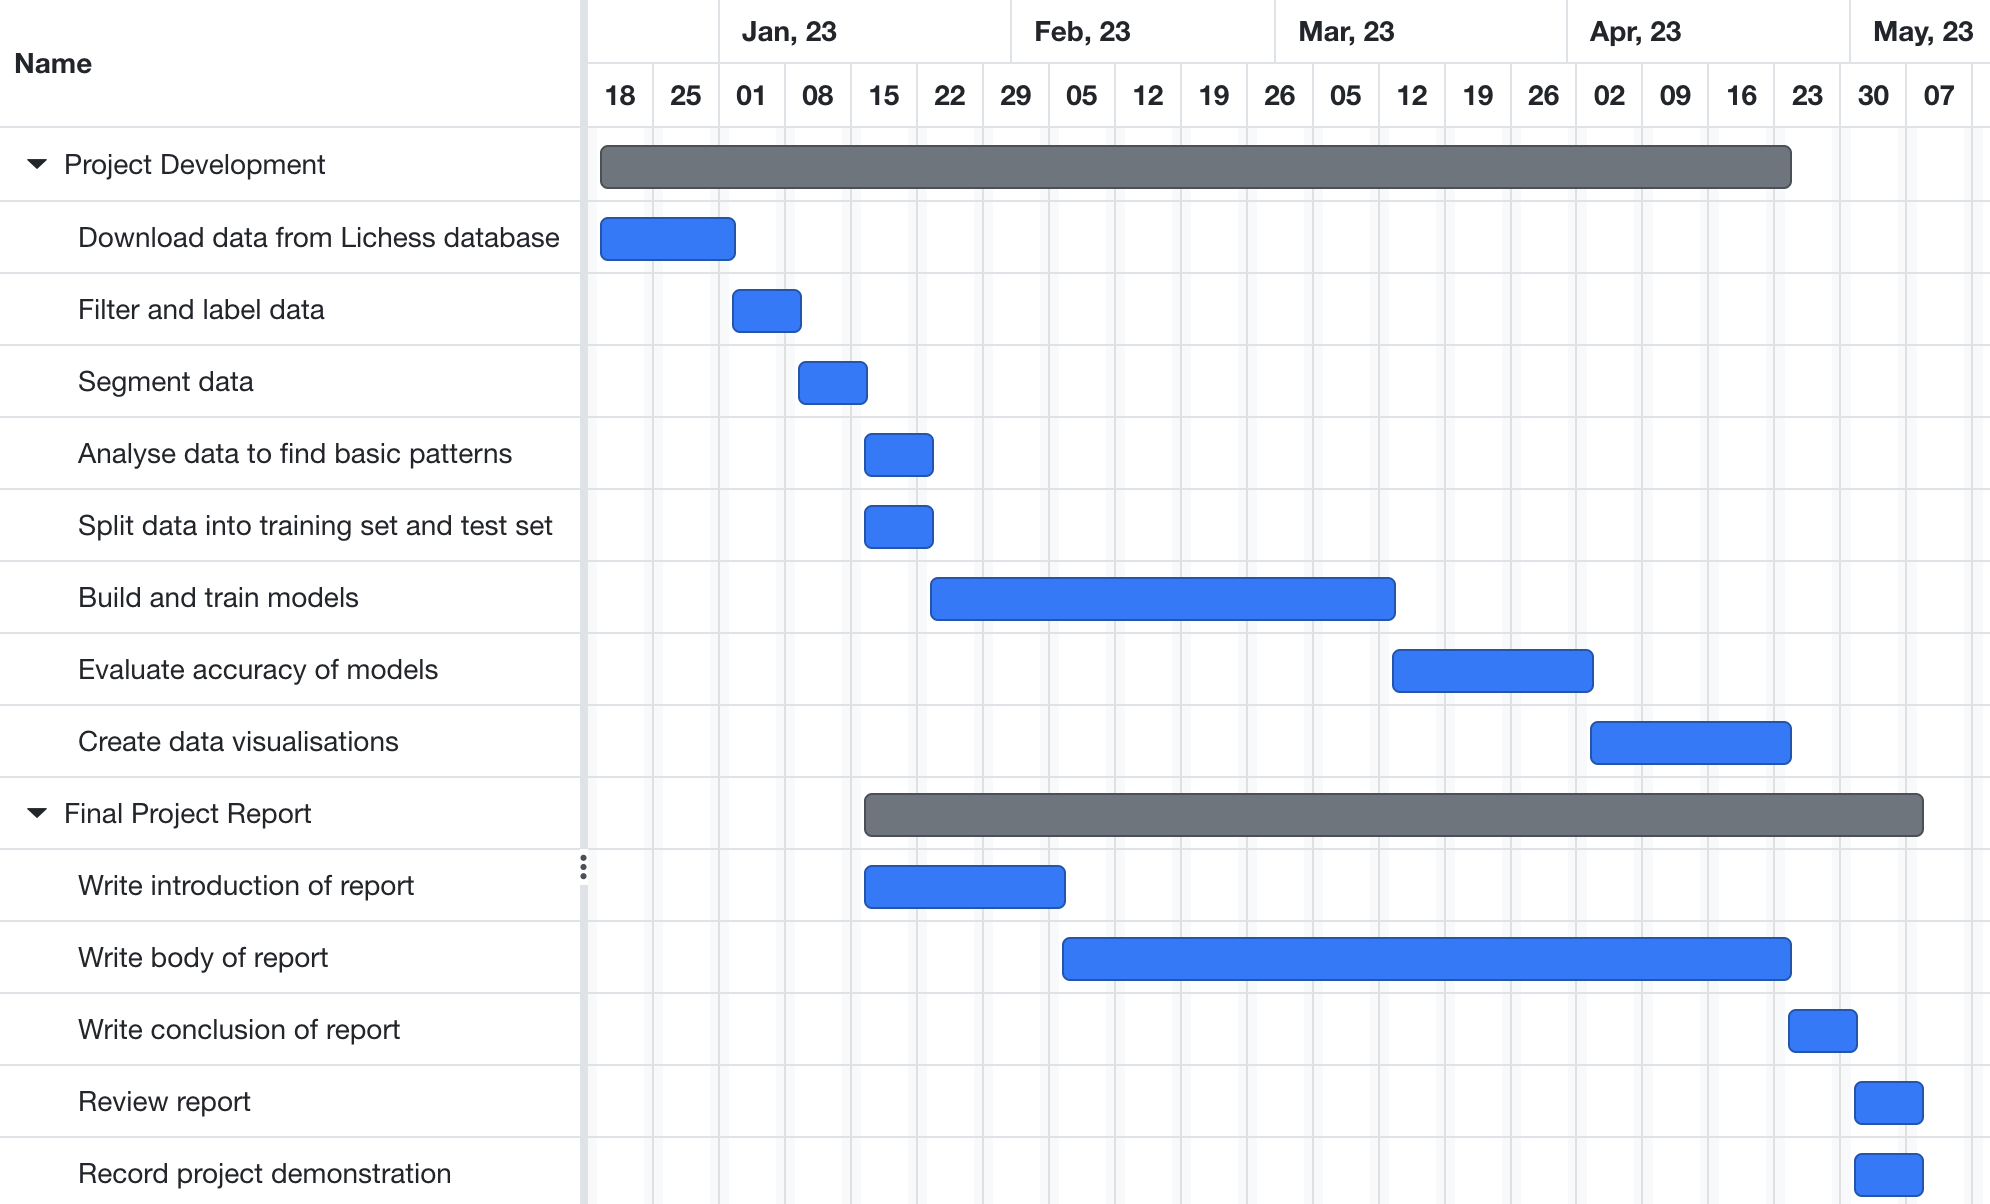
\includegraphics[width=1\textwidth]{images/Gantt Chart - Project Management.png}
    \end{center}
\end{appendices}

\end{document}